\documentclass[11pt]{article}
\usepackage[a4paper, total={6in, 8in}]{geometry}
\usepackage{amsmath}
\usepackage{amsthm}
\usepackage{graphicx}
\usepackage{amsfonts}
\usepackage{xcolor}
\usepackage{enumerate}
\begin{document}

\newtheorem{theorem}{Theorem}
\numberwithin{theorem}{section}
\theoremstyle{definition}
\newtheorem{definition}{Definition}
\newtheorem{proposition}{Proposition}
\newtheorem{example}{Example}
\newtheorem{lemma}{Lemma}
\newtheorem{corollary}{Corollary}
\numberwithin{definition}{section}
\numberwithin{proposition}{section}
\numberwithin{example}{section}
\numberwithin{lemma}{section}
\numberwithin{corollary}{section}
\newcommand{\uw}{\mathcal{U}(W,X)}
\newcommand{\W}{$(W,S)$}
\newcommand{\ix}{\textit}
\newcommand{\tr}{\textcolor{red}}
\newcommand{\sg}{$\Sigma$}


%\title{Buildings}
%\maketitle


\section{Shadows in buildings}

We want to consider 

\subsection{Orientations}

\begin{definition}\cite[?]{SHA}
    An \ix{orientation} $\phi$ of $\Sigma$ is a map from the set of pairs $(p,c)$, where $p$ is a panel and $c$ is an alcove containing $p$, to the set $\{+1,-1\}$. If $\phi (p,c)=+1$, then we say that $c$ is on the $\phi$-\ix{positive side}, otherwise we say that $c$ is on the $\phi$-\ix{negative side}. 
\end{definition}


\begin{example}
    The trivial positive orientation is the map which sends all pairs to $+1$. Similarly, the trivial negative orientation is the map which sends all pairs to $-1$. 
\end{example}

Often, we do not want to have orientations which locally behave like trivial orientations. Hence, we define the following concept:

\begin{definition}\cite[?]{SHA}
    Given an orientation $\phi$ of \sg, we have
    \begin{enumerate}
        \item $\phi$ is \ix{locally non-negative} if, for each panel, there is at least one alcove which is on the $\phi$-positive side.
        \item $\phi$ is \ix{locally non-trivial} if, for every panel, there is exactly one alcove which is on the $\phi$-positive side.
    \end{enumerate}
\end{definition}


There is a natural action of $W$ on the set of all possible orientations of \sg, induced by the action of $W$ on on the alcoves and panels. It is defined as 
\[(x\cdot\phi)(p,c):=(x^{-1}p,x^{-1}c).\]

\begin{definition}\cite[?]{SHA}
    Given an orientation $\phi$ of \sg, we say that $\phi$ is \ix{wall consistent} if, given any wall $H$, for all pairs $c,d$ of alcoves which lie in the same halfspace of $H$, with panels $p$ and $q$ respectively, we have that $\phi(p,c)=\phi(q,d)$. If our orientation is wall consistent, we can then define the \ix{positive side} $H^{\epsilon}$ of $H$ as the half-space such that all alcoves $c$ in $H^{\epsilon}$ have $\phi(p,c)=+1$ for all panels of $c$. Then the \ix{negative side} is defined similarly.
\end{definition}

We want to look at several natural ways to orient a Coxeter complex. First, we will look at an orientation which is derived from either a choice of alcove, or a choice of panel. This orientation works for any Coxeter group.

\begin{definition}\cite[?]{SHA}
    Choose a fixed alcove $c$ in \sg. Now given any alcove $d$, and panel $p$, we define their orientation as $\phi(p,d)=+1$ if and only if $c$ and $d$ lie in the same side of the wall which is spanned by $p$. We call this orientation the \ix{alcove orientation towards c}.
\end{definition}


\begin{definition}\cite[?]{SHA}
    Choose a fixed simplex $b$ in \sg. Now given any alcove $c$, and panel $p$ in $c$, we define their orientation as $\phi(q,c)=+1$ if and only if either $c$ and $b$ lie in the same side of the wall $H$ containing $p$, or if $b$ lies inside $H$. We call this orientation the \ix{simplex orientation towards b}.
\end{definition}
\begin{example}
    Here we see two simplex orientations of an $A_2$ Coxeter complex. In this complex, the alcoves are edges, and the panels are vertices.
\end{example}
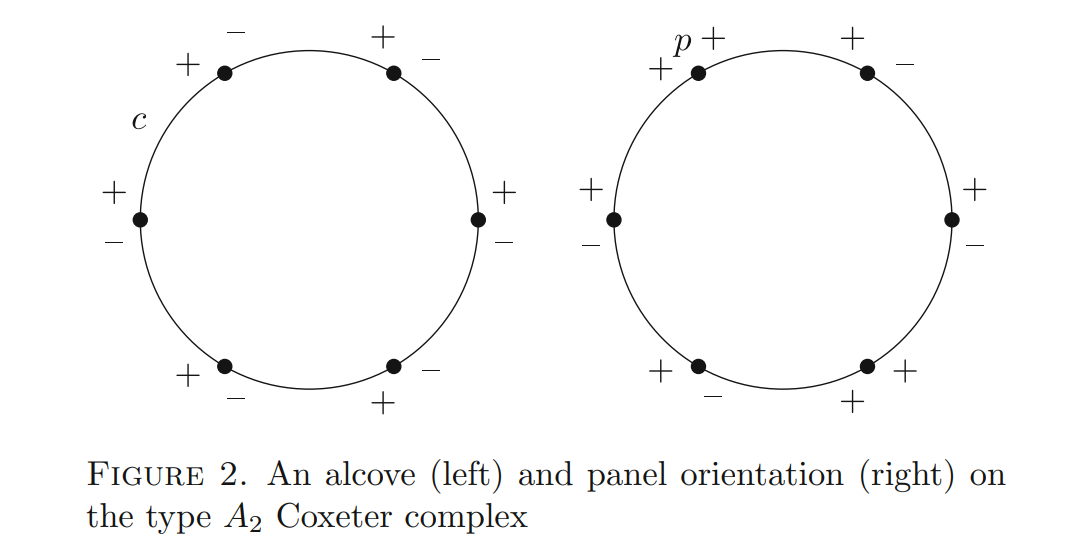
\includegraphics[scale=0.6]{Screenshot 2023-02-03 102201.png}\\

\begin{lemma}\cite[?]{SHA}
    Consider a Coxeter group $(W,S)$ with Coxeter complex \sg. We have the following:
    \begin{enumerate}[(i)]
        \item If $\phi$ is a simplex orientation of \sg, then $\phi$ is wall consistent and locally non-negative.
        \item If $\phi$ is an alcove orientation of \sg, then $\phi$ is wall consistent and locally non-trivial.
    \end{enumerate}
\end{lemma}

\begin{proof}
    (i) Let $b$ be the simplex defining the orientation, and consider a wall $H$ in our Coxeter complex. First let us consider the case in which $b$ lies inside $H$. Then, by definition of the simplex orientation, both sides of the wall are defined to be positive. So any two alcoves, and any respective panels, lying in the same halfplane of $H$ will have the same orientation. So this wall satisfies the conditions of wall consistency, and both sides are defined as positive so it is locally non-negative. 
    
    Now assume that $b$ does not lie in $H$, so $b$ lies in exactly one halfplane of $H$. Then this side of the halfplane is the positive side, and any two alcoves, and any respective panels, in this halfplane are given a positive orientation. Similarly, any two alcoves, and any respective panels, in the other halfplane are given a negative orientation. So again, this wall satisfies the conditions of wall-consistency, and both sides are defined as positive so it is locally non-negative. 

    (ii) An alcove orientation is a type of simplex orientation, so part (i) implies that $\phi$ is wall consistent. Now considering the cases from part (i), we can never be in the first case. This is because an alcove has one higher dimension whan a wall, and so an alcove can never fully lie within a wall. So therefore we are always in case two, and so by the same argument as part (i), we conclude that $\phi$ is locally non-trivial. 
\end{proof}

\subsection{The affine case}

Now we want to consider when our Coxeter complex $\Sigma$ is affine. To define an orientation on \sg, we choose a chamber at infinity.

If $\phi$ is a wall consistent orientation, then, given two chambers $c,d$ which share a common panel $p$, $c$ and $d$ are given the same orientation if they lie in the same half-space of the hyperplane spanned by $p$. This amounts to picking a positive side of the hyperplane.

However, we did not have to pick these positive sides in any consistent way. 

\begin{definition}
    Let $\phi$ be a wall consistent orientation of an affine Coxeter complex. We say that $\phi$ is \ix{periodic} if, given two parallel hyperplanes $H_1,H_2$ and corresponding half-spaces $H_1^{\epsilon},H_2^{\epsilon}$, if $H_1^{\epsilon}\subset H_2^{\epsilon}$, then $H_1^{\epsilon}$ is positive if and only if $H_2^{\epsilon}$ is positive. 
\end{definition}

\begin{example}
    If $\phi$ is a trivial orientation on an affine Coxeter complex, then $\phi$ is periodic. 
\end{example}

\begin{example}
    Simplex orientations are not periodic, as, for every set of parallel hyperplanes, we can find pairs of representatives which have the simplex on different sides.
\end{example}

If $\phi$ is a periodic orientation, then we have a natural orientation induced on the boundary. Similarly, if we have an orinetation defined on the boundary of a Coxeter complex, then we have a periodic orientation on the Coxeter complex which induces this orientation. 

\begin{lemma}\cite[p.125]{SHA}
    Given a periodic orientation $\phi$ on an affine Coxeter complex \sg, there is an induced wall-consistent orientation $\partial\phi$ on the boundary complex $\partial\Sigma$. Now if $\phi$ is locally non-negative or non-trivial, so is $\partial\phi$. 
\end{lemma}

\begin{proof}
    Consider a wall $M$ in the boundary $\partial\Sigma$. This corresponds to a set of parallel walls in $\Sigma$. Consider a chamber $a\in \partial\Sigma$, which has a panal $p$ lying in $M$. Now we can find a Weyl chamber $C_a$ of $\Sigma$ which represents $a$. This has a bounding wall $H_M$ in the set of parallel walls corresponding to $M$. Let $c$ be the alcove at the tip of $C_a$. So $c$ has a panel $q$ which lies in $H_M$. We now define the orientation of the boundary by 
    \[\partial \phi (a,p)= \phi (c,q).\]
    This is well-defined as $\phi$ is periodic, so the choice of $C_a$ does not affect the orientation. Also, as $\phi$ is periodic, this orientation is wall-consistent. 
    If $\phi$ is locally non-negative, then given a panel $p$ of $\Sigma$, we can find an alcove $c$ such that $\phi(c,p)=+1$. Then under the projection map from $\Sigma$ to the boundary $\partial\Sigma$, we get a chamber $d$ and panel $q$ such that $\partial\Sigma(d,q)=+1$. So $\partial\phi$ is locally non-negative. The same argument can be made to show that if $\phi$ is locally non-trivial, then $\partial\phi$ is also locally non-trivial. 
\end{proof}


\begin{lemma}
    Given a wall-consistent orientation $\phi$ of the boundary complex $\partial\Sigma$, there exists a unique periodic orientation $\tilde{\phi}$ of \sg, which induces the orientation $\phi$. 
\end{lemma}

\begin{proof}
    Let $H$ be a wall in $\Sigma$. Given a halfplane $H^\epsilon$ of $H$, we define $H^\epsilon$ to be the positive side of $H$ if the corresponding halfplane $\partial H^\epsilon$ is the positive side of the wall $\partial H$ with respect to the orientation $\phi$. Otherwise we define $H^\epsilon$ to be the negative side of $H$. This is well-defined as $\phi$ is wall-consistent. This definition also uniquely defines the orientation $\tilde{\phi}$. 
\end{proof}

\begin{definition}
    Let $\sigma$ be a chamber of the boundary $\Delta$ of a Coxeter complex \sg. Then we form an orientation $\phi_{\sigma}$ on the boundary $\Delta$. The \ix{Weyl chamber orientation} on $\Sigma$ is the induced orientation by $\phi_{\sigma}$. 
\end{definition}


\section{Folded galleries}

\subsection{Definitions}
\begin{definition}
    Given a Coxeter complex \sg, a \ix{combinatorial gallery} is a sequence
    \[\gamma = (c_0,p_1,c_1,p_2,...,p_n,c_n),\]
    where the $c_i$ are alcoves and the $p_i$ are panels of \sg, such that $p_i$ is contained in $c_i$ and $c_{i-1}$ for all $i-1,...,n$. The length of a combinatorial gallery $\gamma$ is $n+1$ - this counts how many alcoves there are in the sequence. Then $\gamma$ is \ix{minimal} if there does not exist a shorter gallery starting at $c_0$ and ending at $c_n$. 
\end{definition}

So a gallery is a path between $c_0$ and $c_n$ through alcoves, such that adjacent alcoves in the path share a commmon panel. 

\begin{definition}
    Given a gallery $\gamma$ of \sg, we say that $\gamma$ is \ix{folded (or stammering)} if, within $\gamma$, we can find an index $i$ such that $c_i=c_{i-1}$. Then we say that $\gamma$ has a \ix{fold} at panel $p_i$. Otherwise, we say that $\gamma$ is \ix{unfolded (or non-stammering)}.  
\end{definition}

\begin{definition}
    Given a gallery $\gamma$, define the set F$(\gamma)$ to be the subset of $\{1,...,n\}$ such that $i\in$ F$(\gamma)$ if and only if $\gamma$ has a fold at panel $p_i$. 
\end{definition}

To represent a gallery, we draw a path which passes through every chamber and panel in the gallery of the Euclidean representation of our Coxeter complex. We draw an arrow towards the sink of our gallery. 

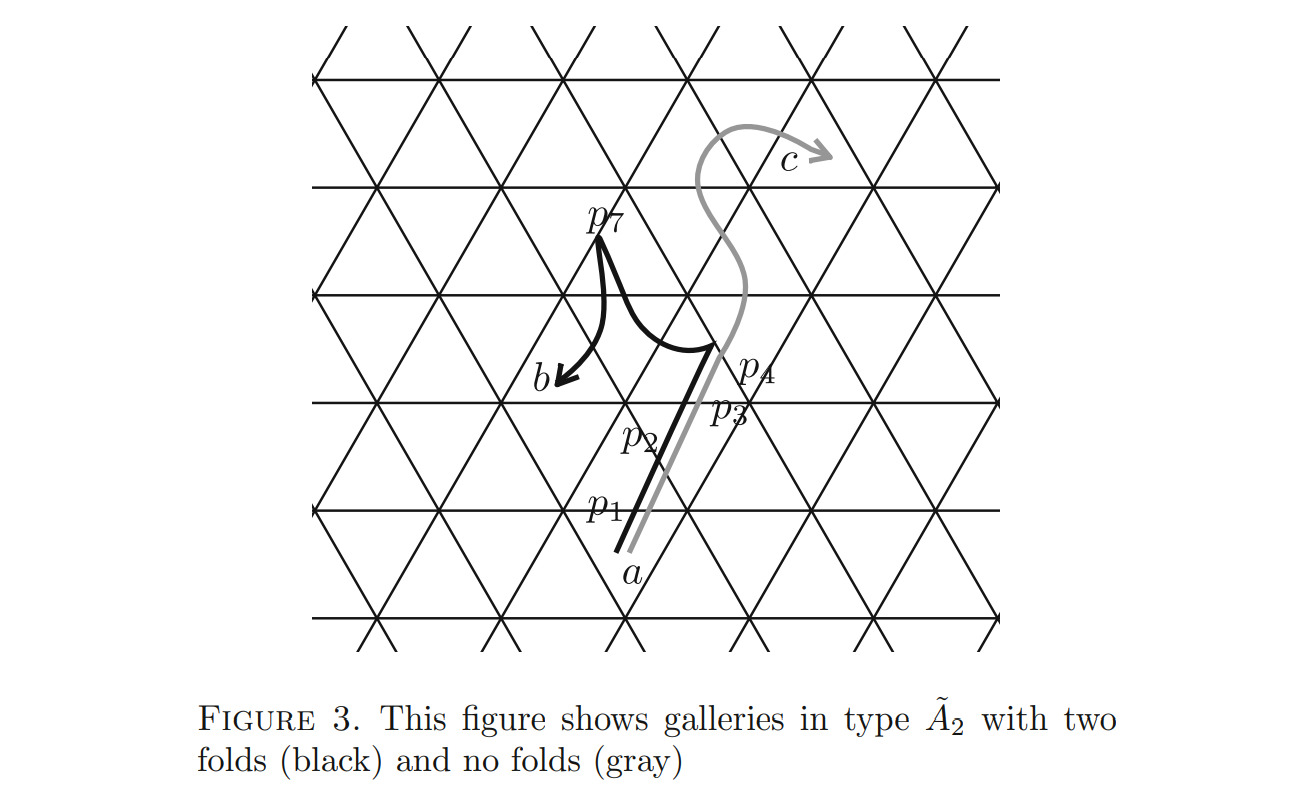
\includegraphics[scale=0.6]{Screenshot 2023-02-03 111653.png}\\

\begin{definition}
    Given a gallery $\gamma$ in \sg, and an orientation $\phi$, we say that $\gamma$ is \ix{positively folded} with respect to $\phi$ if, whenever $\gamma$ is folded at position $i$, $\phi(p_i,c_i)=+1$.  We can similarly define \ix{negatively folded}.
\end{definition}


\subsection{Galleries and Words}

\begin{definition}
    Consider a gallery $\gamma = (c_0,p_1,c_1,...,p_n,c_n)$. Let panel $p_i$ of $\gamma$ have type $s_{j_i}\in S$. We define its \ix{type} $\tau(\gamma)$ as the word 
    \[\tau(\gamma):=s_{j_1}...s_{j_n}.\]
    We denote by $\Gamma_{\phi}^+(w)$ the set of all $\phi$-positively folded galleries which have type $w$. 
\end{definition}

We can now define the type and decorated type of a gallery. Note that here we use tilde notation to denote a decorated word, but in other texts, such as \cite{SHA}, they use hat notation to denote the decorated word.
\begin{definition}
    The \ix{decorated type} $\hat\tau(\gamma)$ of a gallery $\gamma = (c_0,p_1,c_1,...,p_n,c_n)$ is the decorated word
    \[\tilde\tau(\gamma):= s_{j_1}...\tilde{s_{j_i}}...s_{j_n},\]
    where we place a hat on the elements $s_{j_i}$ of the word which correspond to a fold $c_{i-1}=c_i$ of the gallery. We denote by $\Gamma_{\phi}^+(\tilde{w})$ the set of all $\phi$-positively folded galleries which have decorated type $\tilde{w}$.
\end{definition}


\begin{lemma}\cite[p.128]{SHA}
    Let $c_0$ be a fixed alcove in our Coxeter complex \sg. 
    \begin{enumerate}[(i)]
        \item There is a bijection between words in $S$ and unfolded galleries starting at $c_0$.
        \item There is a bijection between decorated words in $S$ and gallleries starting at $c_0$. 
    \end{enumerate}
\end{lemma}

\begin{proof}
    Given a word $s_1...s_n$ in $S$, we can define an unfolded gallery starting at $c_0$ by multiplying $c_0$ by $s_1$, and in general define $c_i$ by multiplying $c_{i-1}$ by $s_{i}$, and set $p_i$ to be the unique panel contained in both $c_{i-1}$ and $c_i$. This gives our bijection for part (i). 
    Now given a decorated word in $S$, we can define a general gallery by multiplying $c_{i-1}$ by $s_{i}$, as above, if $s_{i}$ is not decorated. If $s_{i}$ is decorated, then let $c_i=c_{i-1}$, and let the panel $p_i$ be the unique panel of $c_i$ which has type $s_i$. This gives the bijection for part (ii). 
\end{proof}

The next lemma gives some easy results from the definitions of type and decorated type. 

\begin{lemma}\cite[p.128]{SHA}
    Let $\gamma$ be a gallery. Then
    \begin{enumerate}
        \item $F(\gamma)=\emptyset$ if and only if $\tau(\gamma)=\tilde{\tau}(\gamma).$
        \item $\gamma$ is minimal if and only if $F(\gamma)=\emptyset$ and $\tau(\gamma)$ is reduced.
    \end{enumerate}
\end{lemma}

We want to be able to characterise the last alcove in a gallery. We do this by constructing another gallary which removes any folds from our original gallery. This leads to an unfolded gallery which has shorter length than the original gallery.

\begin{definition}
    Consider a gallery $\gamma = (c_0,p_1,c_1,...,p_n,c_n)$ in \sg. We create a new gallery, called the \ix{footprint} \ix{ft}$(\gamma)$ \ix{of} $\gamma$, by deleting all pairs $p_i,c_i$ such that the letter $s_i$ has a hat in $\hat{\tau}(\gamma)$. 

\end{definition}

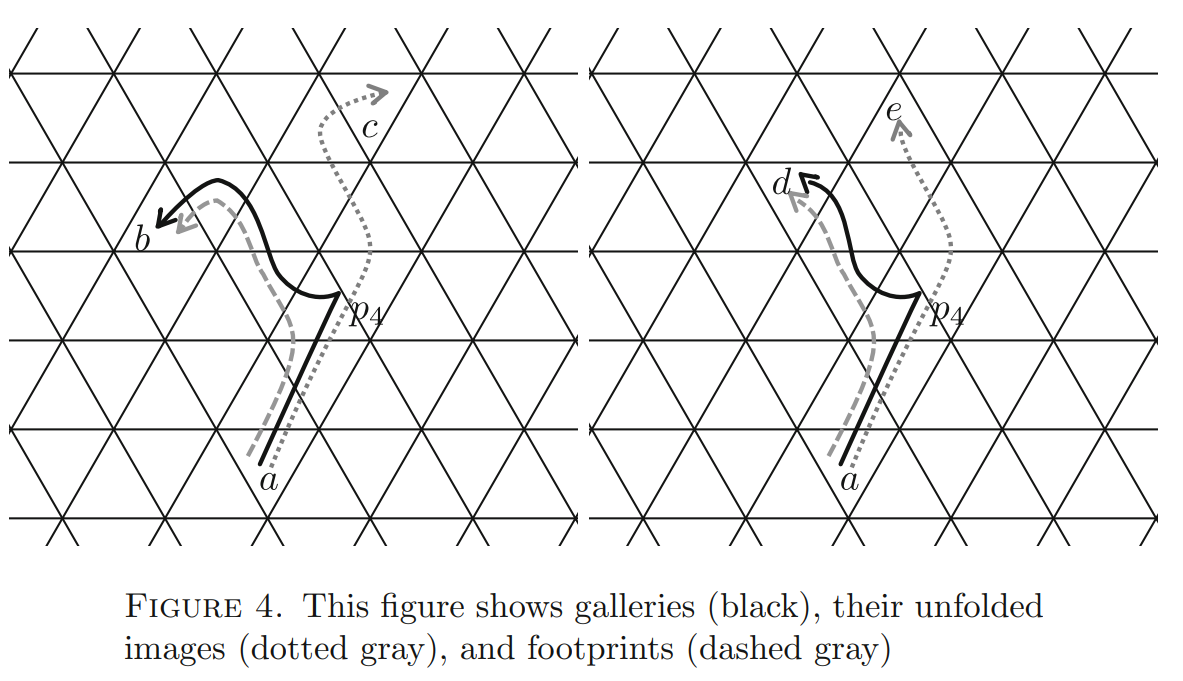
\includegraphics[scale=0.6]{Screenshot 2023-02-03 133522.png}\\

\begin{lemma}
    We can calculate the final alcove of a gallery as the element $c_n=c_0\cdot w$, where $w=\tau(\text{ft}(\gamma))$.
\end{lemma}

\begin{proof}
    The footprint of a gallery is exactly the gallery achieved by deleting repeated alcoves and the corresponding panels. So we are left with a gallery ft$(\gamma)=(c_o=d_0,q_1,d_1,...,q_m,d_m=c_n)$. Now $d_i$ is exactly defined as the alcove obtained by multiplying $d_{i-1}$ by $s_i$, where $s_i$ is the type of the panel $q_i$. So, by induction, $d_m$, which equals $c_n$, can be calculated by multiplying $d_0=c_0$ by the type of ft$(\gamma)$. 
\end{proof}

\subsection{Folding and unfolding galleries}

Now we have defined galleries, and in particular folded galleries, we want to be able to create folded galleries ourselves from unfolded galleries. We do this in a natural way, where folding along a panel leads to a reflection of the rest of the gallery with respect to that panel. For instance, this figure shows foldings in the 4th and 7th panel of the given gallery, and also illustrates that foldings are commutative - a fact that we will formally prove.

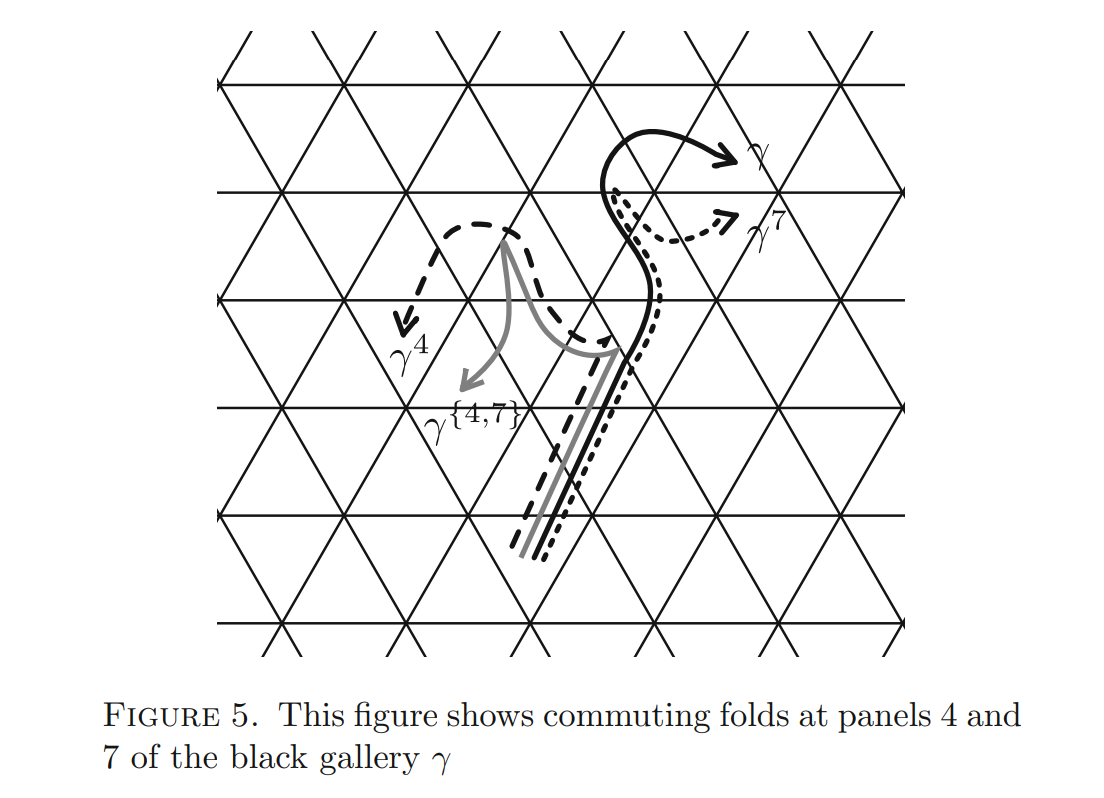
\includegraphics[scale=0.6]{Screenshot 2023-02-03 153412.png}\\

We note that, as $W$ has a natural left action on \sg, $W$ also acts on the set of galleries in \sg. For instance, $x\in W$ sends $\gamma = (c_0,p_1,c_1,...,p_n,c_n)$ to the gallery $\gamma = (xc_0,xp_1,xc_1,...,xp_n,xc_n)$. 

\begin{lemma} MOVE THIS LEMMA
    Consider an affine Coxeter system $(W,S)$ with a Coxeter complex \sg. Let $a$ be a chamber in the boundary complex $\partial\Sigma$. Now a gallery $\gamma$ is $\phi_a$-positively folded if and only if $x\cdot \gamma$ is $\phi_a$-positively folded. So the action of $W$ on $\partial\Sigma$ preserves the condition of being '$\phi_a$-positively folded'.
\end{lemma}

\begin{proof}
    
\end{proof}

\begin{definition}
    Consider a gallery $\gamma = (c_0,p_1,c_1,...,p_n,c_n)$. Let $H_i$ be the hyperplane containing the panel $p_i$, and let $r_i$ be the reflection across $H_i$. For $i=1,...,n$, let
    \[\gamma^i:=(c_o,p_1,...,p_i,r_ic_i,r_ip_{i+1},r_ic_{i+1},...,r_ip_n,r_ic_n).\]
    If $\gamma$ was folded at panel $p_i$, we call $\gamma^i$ a \ix{unfolding of }$\gamma$ at $p_i$. Otherwise, we call it a \ix{folding}.
\end{definition}

\begin{lemma}
    For all $i=1,...,n$, $\tau(\gamma)=\tau(\gamma^i)$. So folding and unfolding does not change the gallery type. Also, $(\gamma^i)^i=\gamma$.
\end{lemma}

\begin{proof}
    This is just a result of the definition of the type of a panel, which is invariant under reflections along walls. Also, we note that $r_ir_i=1$, as reflections are self-inverse, so applying a fold twice at panel $p_i$ will first achieve $(c_o,p_1,...,p_i,r_ic_i,r_ip_{i+1},r_ic_{i+1},...,r_ip_n,r_ic_n)$, and will then achieve $(c_o,p_1,...,p_i,r_ir_ic_i,r_ir_ip_{i+1},r_ir_ic_{i+1},...,r_ir_ip_n,r_ir_ic_n)=(c_0,p_1,...,p_n,c_n)$. Hence, $(\gamma^i)^i=\gamma$.
\end{proof}

\begin{lemma}
    For all $i,j=1,...,n$, $(\gamma^i)^j=(\gamma^j)^i$, i.e. foldings are commutative.
\end{lemma}

\begin{proof}
    As we have already dealt with the case that $i=j$, we can assume that $i<j$. Let $r$ be the reflection along the wall containing $p_i$, and let $t$ be the reflection along the wall containing $p_j$. Then we have, by the definition of (un)-folding,
    \[(\gamma^j)^i=((c_0,p_1,c_1,...,c_{i-1},p_i,rc_i,...,rp_j,rtc_j,...,rtc_n)).\]
    Also, if we let $u$ be the reflection along the wall containing $rp_j$, we have
    \[(\gamma^i)^j=((c_0,p_1,c_1,...,c_{i-1},p_i,rc_i,...,rp_j,urc_j,...,urc_n)).\]
    Let us calculate the maps $r$, $t$ and $u$. Given a panel $p$ of an alocve $c$, the reflection along the wall containing $p$ is given by the multiplication map $c\tau(p)c^{-1}$. Hence,
    \[r=c_{i-1}\tau(p_i)c_{i-1}^{-1}, t=c_{j-1}\tau(p_j)c_{j-1}^{-1}, \textnormal{ and } u=(rc_{j-1})\tau(rp_j)(rc_{j-1})^{-1}.\]
    Now by lemma ..., reflections preserve type, so we have that $\tau(rp_j)=\tau(p_j)$. Then
    \[\begin{aligned}
        ur & =(rc_{j-1})\tau(rp_j)(rc_{j-1})^{-1}c_{i-1}\tau(p_i)c_{i-1}^{-1}\\
           & =r(c_{j-1}\tau(p_j)c_{j-1}^{-1})(c_{i-1}\tau(p_i)c_{i-1}^{-1})(c_{i-1}\tau(p_i)c_{i-1}^{-1})\\
           & = r(c_{j-1}\tau(p_j)c_{j-1}^{-1})\\
           & =rt.
    \end{aligned}\]
    Therefore $ur=rt$, and hence $(\gamma^j)^i=(\gamma^i)^j$.
\end{proof}

Because of this property, we are able to define a \ix{multifolding} with respect to a subset $I$ of $\{1,...,n\}$ as the (un-)foldings $\gamma^I$. Now multifoldng does not affect the type. Then the set of folds of $\gamma^I$ will be the symmetric difference of the folds of $\gamma$ and $I$. In particular, if $I$ and $J$ are subsets of $\{1,...,n\}$, $(\gamma^I)^J=\gamma^{I\Delta J}$. The following corollary now follows.

\begin{corollary}
    Given any gallery $\gamma$, there is a subset $I\subset \{1,...,n\}$ such that $\gamma^I$ is unfolded, and $\gamma$ and $\gamma^I$ have the same type.
\end{corollary}


Now we fix an alcove of our Coxeter complex, and call this 1. Then, for any word $w$ with elements in $S$, we let $\gamma_w$ be the unique unfolded gallery which has type $w$ and starts at 1. Now we write
\begin{enumerate}
    \item $\gamma \rightharpoonup \eta$ if $\gamma$ and $\eta$ are galleries such that $\eta = \gamma^I$ for some index set $I$,
    \item $w\rightharpoonup u$ if $w$ and $u$ are words in $S$ such that there is a folding of $\gamma_w$ which has footprint $u$.
    \item $w\rightharpoonup x$ if $x$ is an element of $W$ such that there is a folding of $\gamma_w$ which has end alcove $c_x$. 
\end{enumerate}
We denote by $A\stackrel{\phi}{\rightharpoonup} B$ if the respective gallery is $\phi$-positively folded.


\section{Braid invariant orientations}

Two reduced words in $S$ represent the same element in the Coxeter group if and only if they differ by a squence of braid moves CITE. A braid move replaces a subword $s_is_j...$ of length $m_{ij}$ with the string $s_js_i...$, again of length $m_{ij}$. We want to define the concept of braid invariant orientations, so we can later conclude that, if we have a braid invariant orientation, our shadows of a gallery do not depend on the chosen word of $S$ representing the end alcove. 

\begin{definition}
    Consider a Coxeter system $(W,S)$ and a corresponding Coxeter complex \sg. Let $\phi$ be an orientation on \sg. Then we say that $\phi$ is \ix{braid invariant} if, given any two braid equivalent words $w,w'$ in $S$ and any $x\in W$, $w\stackrel{\phi}{\rightharpoonup} x$ if and only if $w'\stackrel{\phi}{\rightharpoonup} x$. Then if $y\phi$ is braid invariant for all $y\in W$, $\phi$ is called \ix{strongly braid invariant}. 
\end{definition}

For instance, trivial orientations are strongly braid invariant, but these orientations are not very interesting. The following proposition gives us a large family of orientations which are braid invariant. A proof of this proposition can be found in \cite[pp.135-138]{SHA}.

\begin{proposition}
    Weyl chamber orientations are braid invariant.
\end{proposition}

\tr{Happy to prove this proposition, but the proof is very long so wanted to ask before I wrote it.}

\section{Shadows}
\begin{definition}
    Consider a Coxeter system $W$ and an orientation $\phi$ on the Coxeter complex \sg\W. Let $w$ be a word is $S$. The \ix{shadow} of $w$ with respect to $\phi$ is the set 
    \[\textnormal{Sh}_\phi(w):=\{u\in W|w\stackrel{\phi}{\rightharpoonup} u\}.\]
    If $\phi$ is braid invariant, we can define Sh$_\phi(x)=$Sh$_\phi(w)$, where $w$ is any reduced expression of $x\in W$. If we have the Weyl chamber orientation $\phi_a$ with $a\in W_0$, the \ix{regular shadow} of $x$ with respect to $a$ is Sh$_a(w):=$Sh$_{\phi_a}(w)$. The \ix{full shadow} of $x$ is the union of regular shadows. 
\end{definition}

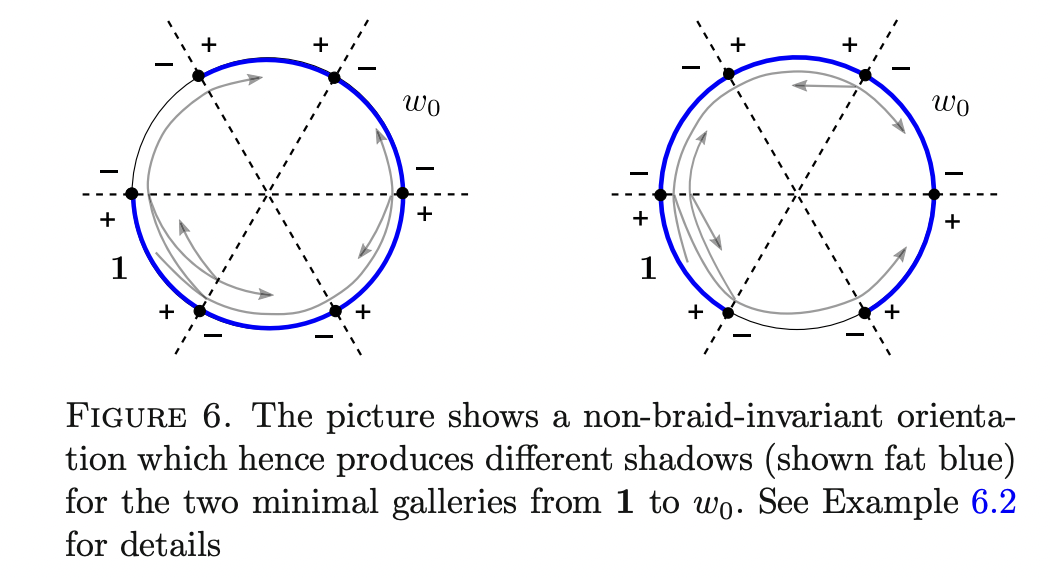
\includegraphics[scale=0.6]{Screenshot 2023-02-08 at 10.39.18.png}\\

\begin{definition}
    Let $x=s_1...s_n$ be a reduced expression for $x\in W$. Let $y\in W$. We say that $y\leq x$ if there exists a reduced expression for $y$ of the form $s_{i_1}...s_{i_k}$ with $1\leq i_1\leq...\leq i_j\leq n$. This ordering is called the \ix{Bruhat order}.
\end{definition}

\begin{proposition}
    Consider the trivial positive orientation $\phi_+$, and the alcove orientation $\phi_1$ towards 1. For $x,y\in W$, $x\geq y$ if and only if $x\stackrel{\phi_+}{\rightharpoonup} y$, if and only if $x\stackrel{\phi_1}{\rightharpoonup} y$.
\end{proposition}

\begin{proof}
    
\end{proof}
\bigbreak
\begin{center}
    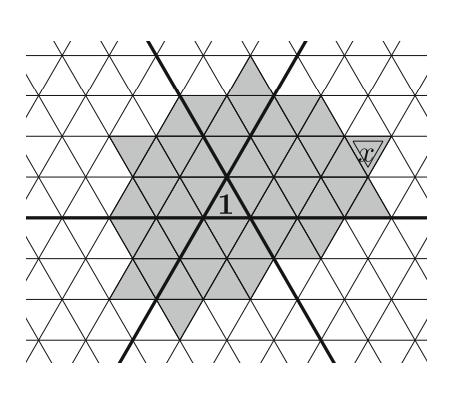
\includegraphics[scale=1]{Screenshot 2023-03-07 133912.png}\\
\end{center}


\begin{example}
    The picture above shows the shadow for an alcove of a Coxeter complex of type $\tilde{A}_2$, with respect to the trivial positive orientation. By the proposition above, this is also the shadow with respect to the alcove orientation towards 1. Furthermore, the alcoves in this shadow are all the elements $y$ of the Coxeter group such that $y\leq x$, and so it is the Bruhat interval $[1,x]$. 
\end{example}













\bibliographystyle{plain}
\bibliography{references}



\end{document}